\documentclass[a4paper,11pt,dvipdfmx]{jsarticle}

\usepackage{bm}
\usepackage[dvipdfmx]{graphicx}
\usepackage[subrefformat=parens]{subcaption}
\usepackage[dvipdfmx]{color}
\usepackage{ascmac}
\usepackage{siunitx}
\usepackage{otf}
\pagestyle{plain}
\usepackage{float}
\usepackage[dvipdfmx]{hyperref}
\usepackage{pxjahyper}
\usepackage{here}
\usepackage{titlesec}
\titleformat*{\section}{\LARGE\bfseries}
\titleformat*{\subsection}{\normalsize\bfseries}
\usepackage{url}
\usepackage{comment}
\usepackage[table,xcdraw]{xcolor}
\hypersetup{% hyperrefオプションリスト
setpagesize=false,
 bookmarksnumbered=true,%
 bookmarksopen=true,%
 colorlinks=true,%
 linkcolor=blue,
 citecolor=blue,
}

\begin{document}


\subsection{検出過程}
散乱した粒子はPINフォトダイオードに入射しエネルギーを落として電流に変換される。本研究ではPINフォトダイオードからの電流がチャージアンプ・オペアンプに入り、シェーパーに入ることによって散乱粒子・反跳粒子を検出した。本研究ではADCとMCAを利用して波高を読むためチャージアンプ出力をシェーピングする必要があった。そのためシェーパーを利用した。利用したシェーパーは豊伸電子製N012である。

\subsubsection{PINフォトダイオード}
一般的にフォトダイオードというのは、半導体のPN接合部に光を照射すると電流や電圧を発生する受光素子である。検出から電気信号への変換効率が良いため、エネルギー分解能が良いという利点がある。PINフォトダイオードは、PN接合部の間にI型半導体を挟んだ検出器である。外部からの逆バイアス電圧が必要だが、空乏層が広くなるため、陽子のエネルギーを確実に落とし切れるという利点がある。\cite{pin}

 \begin{figure}[H]
    \centering
    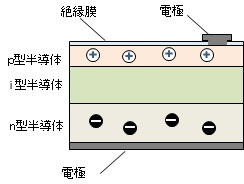
\includegraphics[width=50mm]{picture/setup/pinmoshi.png}
    \caption{PINフォトダイオードの模式図\cite{pin}}
    \label{pin1}
  \end{figure}

逆バイアス電圧がかけられたPINフォトダイオードに、陽子が入射すると、そのエネルギーによってI型半導体内で電離が発生する。I型半導体に電圧をかけることによってできた電界によって図\ref{pin2}のように電子とホールが移動し、電流が流れる仕組みとなっている。この電荷量の測定を行い入射粒子のエネルギーを推定できる。I型半導体の部分がSiの場合、電離する電子-ホール対を1組作成するには300Kで3.62eV必要なため、3MeV程度の散乱陽子ならば、およそ10$^\text{6}$組の対を生成することになる。よって、測定される電荷量が素電荷の値に生成される電子-ホール対の数をかけて、およそ0.16pCになる\cite{2019}。

\par
本実験で用いたPINフォトダイオードは、浜松ホトニクス製のS3590-09である。

 \begin{figure}[H]
    \centering
    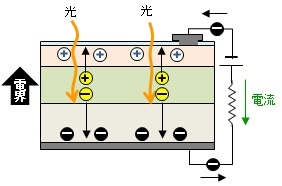
\includegraphics[width=50mm]{picture/setup/pinmoshi2.png}
    \caption{PINフォトダイオードによるエネルギー測定\cite{pin}}
    \label{pin2}
  \end{figure}

\subsubsection{チャージアンプ・オペアンプ}
PINフォトダイオードから流れた電荷信号は、オペアンプによって増幅され、チャージアンプによって電圧信号に変換される。チャージアンプの回路図を図\ref{kairo}に、チャージアンプの写真を図\ref{tya-jianpu}に示す。オペアンプはチャージアンプ回路に含まれており、クリアパルス製CS-515を利用している。本実験では、散乱粒子と反跳粒子の両方を観測したいため、先行研究\cite{2019}で利用していたチャージアンプ回路をもう1つ作成した。また、チャージアンプ回路単体では真空チェンバー内に置くことが不可能であるため、先行研究で利用していたPINフォトダイオード固定台をもう1つ作成し、利用した。PINフォト固定台の写真を図\ref{koteidai}に示す。

 \begin{figure}[H]
    \centering
    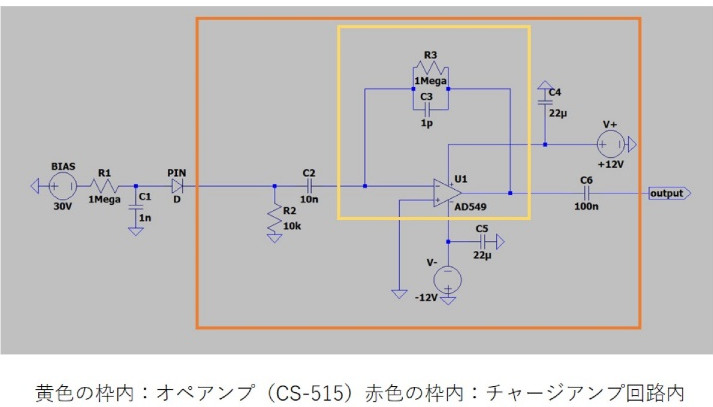
\includegraphics[width=80mm]{picture/setup/kairo.png}
    \caption{チャージアンプ回路図}
    \label{kairo}
  \end{figure}
  
  \begin{figure}[H]
   \begin{minipage}{0.32\linewidth}
    \centering
    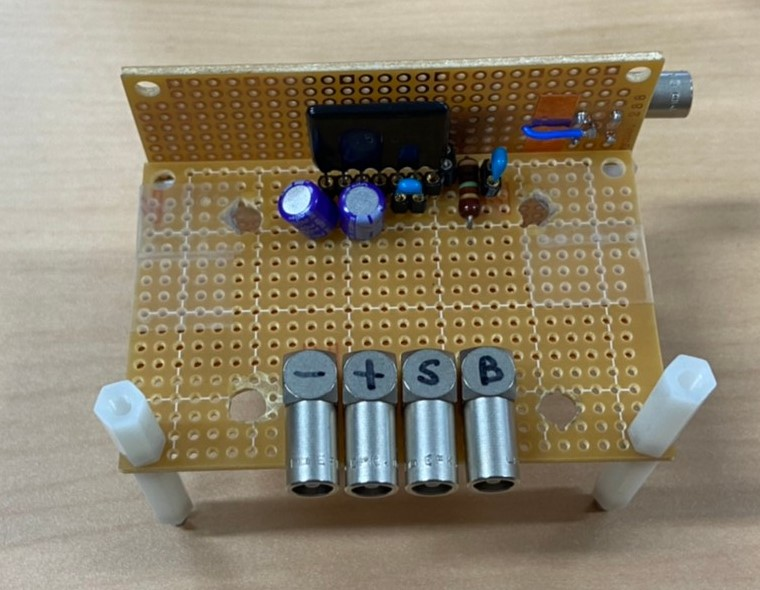
\includegraphics[width=30mm]{picture/setup/omote.jpg}
    \label{omote}
   \end{minipage}
   \begin{minipage}{0.32\linewidth}
    \centering
    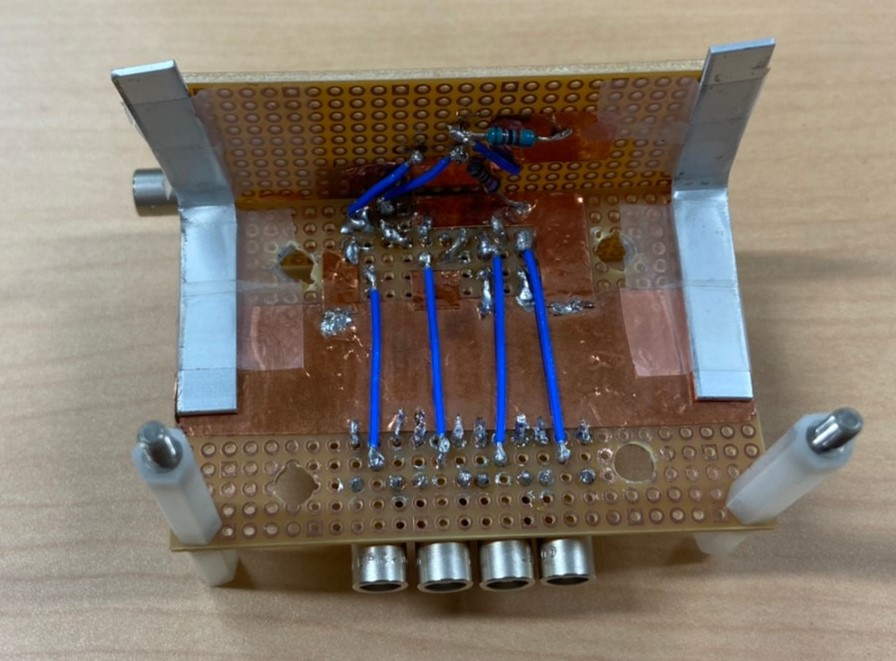
\includegraphics[width=30mm]{picture/setup/ura.jpg}
    \label{ura}
   \end{minipage}
   \begin{minipage}{0.32\linewidth}
    \centering
    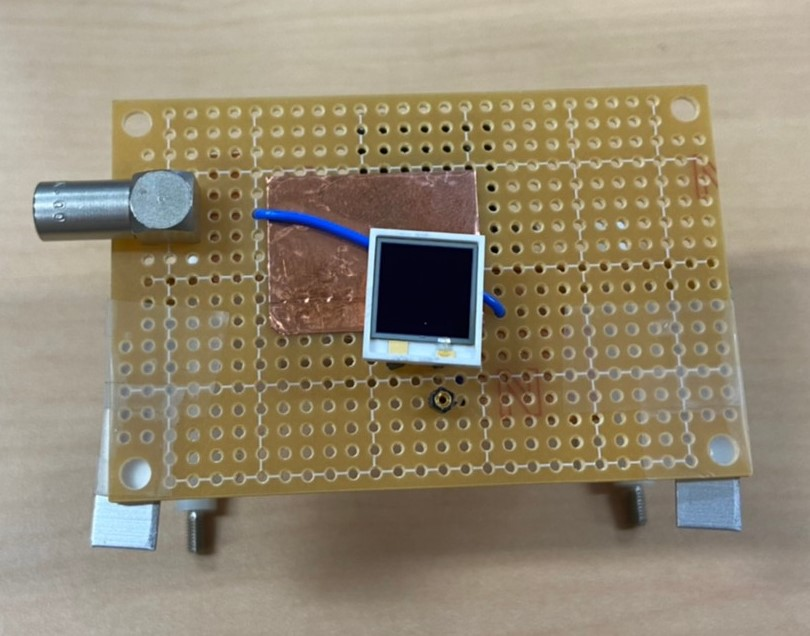
\includegraphics[width=30mm]{picture/setup/sokumen.jpg}
    \label{sokumen}
   \end{minipage}
  \caption{チャージアンプの写真}
  \label{tya-jianpu}
\end{figure}

 \begin{figure}[H]
    \centering
    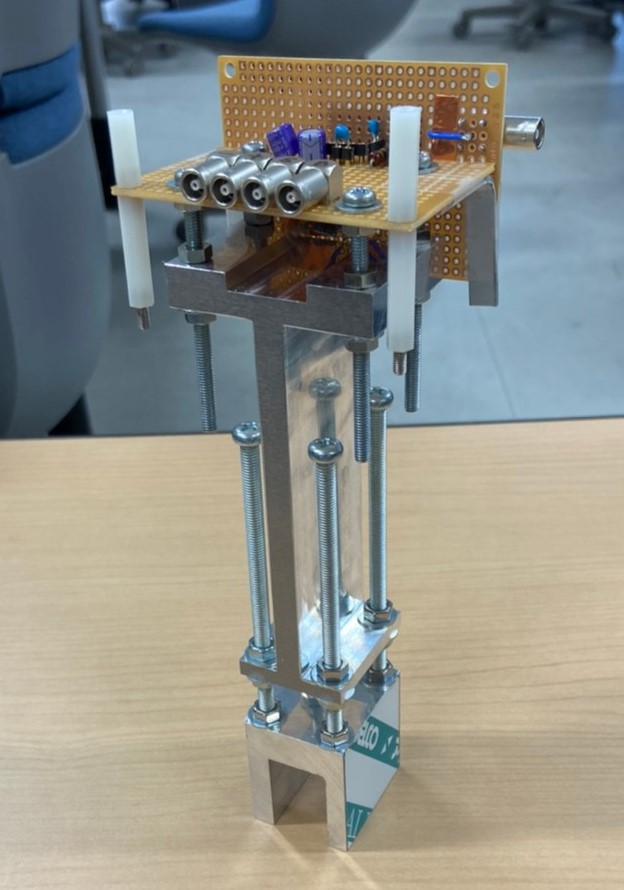
\includegraphics[width=40mm]{picture/setup/koteidai.jpg}
    \caption{PINフォト固定台の写真}
    \label{koteidai}
  \end{figure}
  
\end{document}